\documentclass{article}
\input{setup.tex}
\pagecolor{white}
\numberwithin{equation}{section} % Equations are numbered per section

\title{\Huge \textbf{Computer Vision}
    \\\Large{Nicola Conci
    \\a.y. 2025/2026
    \\University of Trento\\[2cm]}}
\author{Davide Donà}
\date{
    \MonthName\ \number\year \\[0.5em]
    \small\textcolor{gray}{\href{https://github.com/446f6e6e79/computer-vision}{Notes Repository}}
}
\begin{document}
% Set the page numbering to roman numerals
\pagenumbering{roman}

% Title and table of contents
\maketitle

\begin{center}
Computer Vision is the science and technology of machines that \textbf{see}, where
"see" means being able to extract information from an image, necessary to perform a task.
\end{center}

\newpage
\tableofcontents
\newpage
% Change the page numbering to arabic
\pagenumbering{arabic}
\include{chapters/01_image-videos}
\include{chapters/02_elaboration}
\include{chapters/03_models}
\include{chapters/04_motion-detection}
\section{Motion Tracking}
While motion detection identifies the presence of movement, \textbf{motion tracking} aims to 
follow specific objects across consecutive frames. 
This process involves establishing temporal correspondence by associating detected entities in the current 
frame with their instances in subsequent frames, allowing us to reconstruct the trajectory of each object over time.

Motion tracking is essential across various domains, including:
\begin{itemize}
    \item \textbf{People monitoring:} analyzing crowd dynamics or tracking a specific individual;
    \item \textbf{Vehicle tracking:} monitoring the movement of vehicles in traffic surveillance;
    \item \textbf{Biological applications:} tracking the movement of animals or cells in scientific research;
\end{itemize}

The primary objective is often \textbf{object tracking}, which maintains the persistent identity of a target over time. 
Depending on the application, tracking can be performed in different dimensionality:
\begin{itemize}
\item Tracking 2D coordinates in the image plane (e.g., using bounding boxes or centroids);
\item Tracking 3D coordinates in real-world space (requires multiple cameras or depth sensors);
\item Determining the pose or articulation of complex objects, such as human skeletal tracking.
\end{itemize}

\subsection{Foundations: Detection, Association, and Challenges}
Before diving into specific tracking methodologies, it is crucial to understand how raw pixel changes are converted into trackable objects, how these objects are linked across frames, and the common challenges that arise during this process.

\subsubsection{Blob Extraction and Post-Processing}
Following motion detection, the resulting binary masks often contain "noise"—fragmented regions, 
isolated pixels, or holes within moving objects caused by imperfect segmentation. 
To transform these raw pixels into actionable data, we perform \textbf{blob extraction} (also known as Connected Component Labeling).

This process aggregates neighboring foreground pixels into coherent, 
labeled regions called \textbf{blobs}, which represent the physical objects in the scene. 
To ensure these blobs accurately reflect the geometry of the targets, the extraction process typically involves the following refinement steps:
\begin{itemize}
    \item \textbf{Morphological Filtering:} Applying \textit{erosion} to remove isolated noise (small pixel clusters) and \textit{dilation} to bridge gaps and fill internal holes within an object.
    \item \textbf{Connectivity Analysis:} Grouping pixels based on 4-way or 8-way adjacency to assign a unique ID to each spatially distinct moving entity.
    \item \textbf{Feature Extraction:} Once a blob is defined, we calculate its geometric properties, such as the \textbf{centroid}, \textbf{bounding box}, \textbf{area}, and \textbf{aspect ratio}.
\end{itemize}
By filtering out blobs that are too small to be objects of interest, we provide the downstream tracking algorithms with a clean, high-level representation of the scene.

\subsubsection{Target Association}
Once we have the blobs representing the detected objects, we need to associate them across consecutive frames to maintain the identity of each object over time.
This process is known as \textbf{target association} and is actually common to all tracking methods.

In general, detection is not carried out on a frame-by-frame basis, but rather on a \textbf{temporal window} of frames, since it can
be demanding in terms of computational resources. 
This means that the tracking algorithm must be able to handle cases where an object is not detected in every single frame, which adds complexity to the association process.

Correspondence is typically achieved through \textbf{data association algorithms} that match the detected blobs based on their spatial proximity and appearance features.
Such methods rely on the \textbf{optical flow} assumption, which states that the motion of objects between frames is small enough to allow for reliable matching based on their positions and appearances. 
It's important to keep in mind that cameras and frame rates must be chosen to satisfy this assumption, as large displacements can lead to tracking failures.

Different approaches to target association include:
\begin{itemize}
    \item \textbf{Nearest Neighbor:} Assigning each detected blob to the closest track based on spatial distance between centroids;
    \item \textbf{Overlapping:} Matching blobs based on the degree of overlap between their bounding boxes. 
    This has issues with scale changes;
    \item \textbf{Bounding Box - Overlap:} Similar to the previous method, but consider the bounding box of the track instead of the blob.
\end{itemize}
There are no best practices for target association, and the choice of method depends on the specific application and the characteristics of the scene being analyzed.

\subsubsection{Splitting and Merging}
Very similar but distinct problems that can arise during tracking are \textbf{splitting} and \textbf{merging}.

\paragraph{Splitting}
When multiple blobs are present in the same frame, we might encounter one of two problematic scenarios:
\begin{enumerate}
    \item \textbf{Single object - multiple blobs:} this occurs when an object is fragmented into several blobs due to imperfect segmentation.
    \item \textbf{Multiple objects - single blob:} this happens when two or more objects are merged into a single blob, often due to occlusion or proximity.
\end{enumerate}
These 2 situations are different faces of the same problem, which is called \textbf{splitting}. 
\begin{comment}
    #TODO: insert image here for example 1 and 2 from slides
\end{comment}
Before understanding which of the two cases we are facing, evidence need to be collected over a temporal window of frames.
This way, we can analyze the behavior of the blobs over time to determine whether they represent a single object or multiple objects.

\paragraph{Merging}
On the other hand, \textbf{merging} occurs when multiple objects are detected as a single blob, due to proximity or occlusion.
An example of this is when a person which is entering a scene. Initially, feet and arms might be detected as separate blobs.
As the person moves further into the scene, these blobs might merge into a single blob representing the whole body.
\begin{comment}
    #TODO: insert image here for example of merging from slides
\end{comment}

In both cases, its required to analyze the temporal evolution of the blobs to determine whether they represent a single object or multiple 
objects, and to adjust the tracking accordingly.

\subsubsection{Occlusion}
Moving object can be partially or fully occluded by each other when they are in close proximity.
This can lead to tracking failures, as one object disappears from the scene, and bigger blobs may appear, which
might have no resemblance to the original objects.

This is something that need to be handled before the occlusion occurs, by analyzing the proximity 
of the objects and predicting potential occlusions. 

Usually, the system suspends the tracking of the involved objects during the occlusion, and then re-identifies
them once they reappear as separate entities in the scene.

\subsection{2D Tracking Methodologies}
In scenes with a single moving object, tracking can often be achieved by simply following the object's centroid. 
However, multi-object scenarios require sophisticated association algorithms to prevent identity switches. 
Common 2D tracking approaches include:
\begin{itemize}
    \item \textbf{Region-based:} Associating areas based on global features like color or texture.
    \item \textbf{Contour-based:} Tracking the object's based on the shape of its boundary.
    \item \textbf{Feature-based:} Tracking distinct interest points, such as Harris corners or SIFT features.
    \item \textbf{Template-based:} Matching a predefined visual patch of the target across frames.
\end{itemize}

\subsection{Region-Based Tracking}
Region-based tracking follows image patches with a \textbf{uniform appearance}. 
This method is computationally efficient and well-suited for real-time systems, providing a robust balance
between speed and discriminative power.

The standard implementation utilizes a \textbf{color histogram} as a visual signature. 
The workflow typically involves:
\begin{enumerate}
    \item Segmenting the region of interest (ROI) from the background.
    \item Computing the color distribution (histogram) of the ROI.
    \item Searching for the most similar histogram in the subsequent frame to locate the object.
\end{enumerate}

While effective for targets with distinctive colors (each object needs to have a unique color distribution), this approach is sensitive to illumination changes. 
To mitigate this, practitioners often employ the \textbf{HSV color space} (which separates luminance from chromaticity) 
or implement \textbf{dynamic model updates} to adapt the histogram over time.

\subsubsection{Part-Based Models}
A single global histogram may fail when tracking complex, non-rigid objects like humans. 
\textbf{Part-based models} decompose the object into several sub-regions (e.g., head, torso, and legs), 
each with its own local histogram.

This decomposition provides two major advantages:
\begin{itemize}
    \item \textbf{Robustness to Occlusion:} If the legs are hidden by an obstacle, 
    the system can maintain the track using the head and torso signatures.
    \item \textbf{Spatial Verification:} It prevents confusion between objects with similar colors but different 
    configurations. Take in consideration the case of two people, one wearing a white shirt and black pants, 
    and the other wearing a black shirt and white pants. A global histogram might struggle to differentiate them, 
    but a part-based model can leverage the spatial arrangement of colors to maintain accurate tracking.
\end{itemize}

\subsubsection{Implementation and Similarity Metrics}
The tracking process evaluates the similarity between the \textbf{tracked model} ($O^t$) 
in the current frame and a stored \textbf{reference model} ($O^r$), which is updated over time to adapt to changes in the object's appearance.

Common metrics for histogram comparison include:
\begin{itemize}
    \item \textbf{Histogram Intersection:} Measures the correlation between two distributions.
    $$\cap (O^t, O^r) = \sum_{n=1}^{U} \min(O^t_{n}, O^r_{n})$$
    This simply returns the area of the intersection of the two histograms, which is a measure of their similarity.
    \item \textbf{Sum of Squared Differences (SSD):} Measures the Euclidean distance between histogram bins.
    $$SSD(O^t, O^r) = \sum_{n=1}^{U} (O^t_{n} - O^r_{n})^2$$
    This instead returns the area of the difference between the two histograms, which is a measure of their dissimilarity.
\end{itemize}

\begin{center}
    \begin{minipage}{0.48\textwidth}
        \centering
        \resizebox{\linewidth}{!}{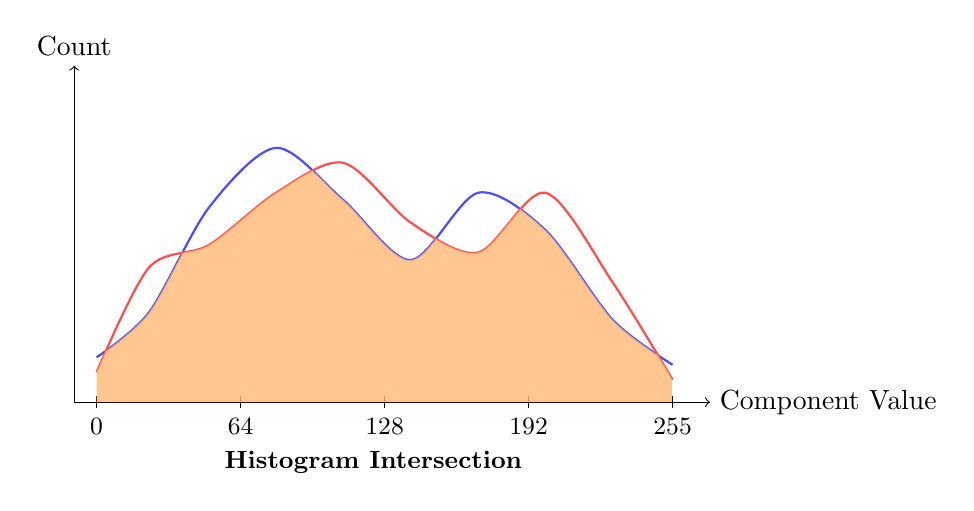
\begin{tikzpicture}[scale=0.95]
    % Axes
    \draw[->] (0,0) -- (8.5,0) node[right] {Component Value};
    \draw[->] (0,0) -- (0,4.5) node[above] {Count};

    % X-axis ticks (0--255 scale)
    \foreach \x/\label in {
        0.3/0,
        2.225/64,
        4.15/128,
        6.075/192,
        8/255
    }{
        \draw (\x,0.08) -- (\x,-0.08);
        \node[below] at (\x,-0.08) {\small \label};
    }

    % Blue histogram curve
    \draw[blue!70, thick]
    plot[smooth]
    coordinates {
    (0.3,0.6) (1,1.2) (1.8,2.6)
    (2.7,3.4) (3.6,2.7) (4.5,1.9)
    (5.4,2.8) (6.3,2.3) (7.2,1.1)
    (8,0.5)
    };

    % Red histogram curve
    \draw[red!70, thick]
    plot[smooth]
    coordinates {
    (0.3,0.4) (1,1.8) (1.8,2.1)
    (2.7,2.8) (3.6,3.2) (4.5,2.4)
    (5.4,2.0) (6.3,2.8) (7.2,1.6)
    (8,0.3)
    };

    % Intersection fill
    \begin{scope}
    \clip
    plot[smooth]
    coordinates {
    (0.3,0.6) (1,1.2) (1.8,2.6)
    (2.7,3.4) (3.6,2.7) (4.5,1.9)
    (5.4,2.8) (6.3,2.3) (7.2,1.1)
    (8,0.5)
    }
    -- (8,0) -- (0.3,0) -- cycle;

    \fill[orange!55, opacity=0.8]
    plot[smooth]
    coordinates {
    (0.3,0.4) (1,1.8) (1.8,2.1)
    (2.7,2.8) (3.6,3.2) (4.5,2.4)
    (5.4,2.0) (6.3,2.8) (7.2,1.6)
    (8,0.3)
    }
    -- (8,0) -- (0.3,0) -- cycle;
    \end{scope}

    % Caption
    \node[font=\small] at (4,-0.8)
    {\textbf{Histogram Intersection}};
\end{tikzpicture}}
    \end{minipage}
    \hfill
    \begin{minipage}{0.48\textwidth}
        \centering
        \resizebox{\linewidth}{!}{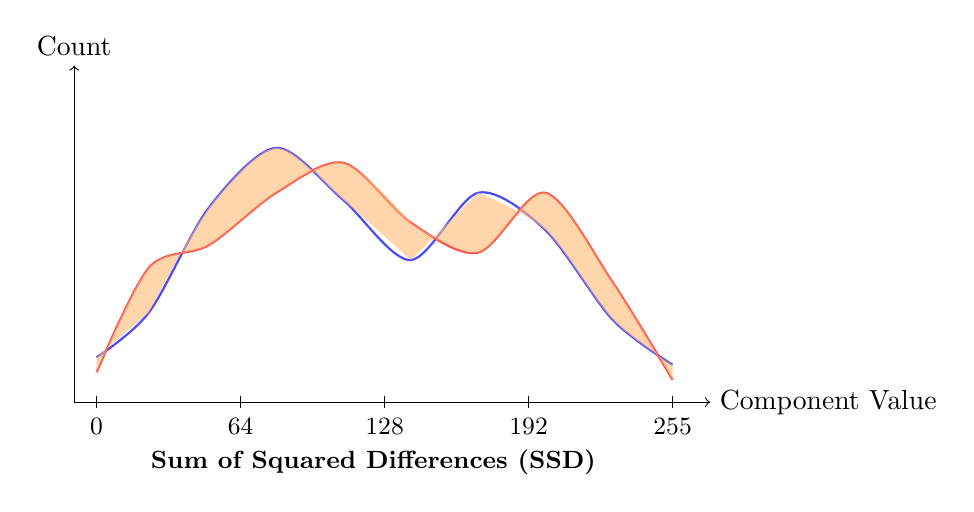
\begin{tikzpicture}[scale=0.95]
    \draw[->] (0,0) -- (8.5,0) node[right] {Component Value};
    \draw[->] (0,0) -- (0,4.5) node[above] {Count};

    \foreach \x/\label in {
        0.3/0,
        2.225/64,
        4.15/128,
        6.075/192,
        8/255
    }{
        \draw (\x,0.08) -- (\x,-0.08);
        \node[below] at (\x,-0.08) {\small \label};
    }

    \draw[blue!70, thick]
    plot[smooth]
    coordinates {
    (0.3,0.6) (1,1.2) (1.8,2.6)
    (2.7,3.4) (3.6,2.7) (4.5,1.9)
    (5.4,2.8) (6.3,2.3) (7.2,1.1)
    (8,0.5)
    };

    \draw[red!70, thick]
    plot[smooth]
    coordinates {
    (0.3,0.4) (1,1.8) (1.8,2.1)
    (2.7,2.8) (3.6,3.2) (4.5,2.4)
    (5.4,2.0) (6.3,2.8) (7.2,1.6)
    (8,0.3)
    };

    \fill[orange!55, opacity=0.6]
    (0.3,0.6)
    -- plot[smooth]
    coordinates {
    (1,1.2) (1.8,2.6)
    (2.7,3.4) (3.6,2.7)
    (4.5,1.9)
    }
    -- plot[smooth]
    coordinates {
    (4.5,2.4) (3.6,3.2)
    (2.7,2.8) (1.8,2.1)
    (1,1.8) (0.3,0.4)
    }
    -- cycle;

    \fill[orange!55, opacity=0.6]
    (4.5,1.9)
    -- plot[smooth]
    coordinates {
    (5.4,2.8) (6.3,2.3)
    (7.2,1.1) (8,0.5)
    }
    -- plot[smooth]
    coordinates {
    (8,0.3) (7.2,1.6)
    (6.3,2.8) (5.4,2.0)
    (4.5,2.4)
    }
    -- cycle;

    \node[font=\small] at (4,-0.8)
    {\textbf{Sum of Squared Differences (SSD)}};
\end{tikzpicture}}
    \end{minipage}
\end{center}

To improve robustness and reduce computational cost, bins typically represent color ranges rather than individual 
values. This is done by grouping pixel values into discrete intervals (e.g., 16 or 32 bins per channel), which allows 
for a more compact representation of the color distribution while still capturing essential information for tracking.

\subsubsection{Addressing Environmental Noise: Shadows}
Shadows represent a significant challenge in region-based tracking because 
they alter the pixel values of the background, often leading to false positives in motion detection. 

To prevent a shadow from being tracked as a separate entity or distorting the object's histogram, 
we assume that a shadow primarily reduces \textbf{brightness} while leaving \textbf{chromaticity} (Hue and Saturation) relatively intact. 
By performing tracking in the HSV space and ignoring the Value ($V$) component, 
the system can become significantly more shadow-invariant, improving the robustness of the tracking process in outdoor 
environments or scenes with variable lighting conditions.

\subsection{Feature Based Tracking}
The idea behind feature-based tracking is to replace the information carried by the histogram of the whole object 
with a set of distinctive local \textbf{features}, extracted from the object itself.
These features are typically points of interest, such as corners, edges, or blobs, that can be reliably detected and tracked across frames.

Considering a set of images $A = \{I_1, I_2, ..., I_n\}$, we can extract a set of features $F_i$ from each image $I_i$.
The position of each feature in a given image can be represented as a vector of coordinates $f_i(x_i, y_i)$.
The objective of feature-based tracking is to determine the displacement vector $d_i = (dx_i, dy_i)$ that best estimates the movement of
feature $f_i$ from one frame to the next, such that:
$$f_{i+1}(x_i + dx_i, y_i + dy_i)$$

\subsubsection{Good Features to Track}
Not all features are equally suitable for tracking. 
The \textbf{Good Features to Track} algorithm identifies features that are likely to be stable and distinctive across frames, making them ideal candidates for tracking.
This method is based on the concept of \textbf{corner detection}, which identifies points in the image where the intensity changes significantly in multiple directions.

For each pixel in the image $p(x, y)$ we compute the \textbf{structure tensor} $Z$:
$$Z = \begin{bmatrix}
    \sum_{W} J_x^2 & \sum_{W} J_x J_y \\
    \sum_{W} J_x J_y & \sum_{W} J_y^2
\end{bmatrix}$$
where $J_x$ and $J_y$ are the gradients of the image in the x and y directions, respectively, 
and the summation is performed over a window $W$ centered around the pixel $p$.

The eigenvalues of the structure tensor, $\lambda_1$ and $\lambda_2$, provide a measure of the local intensity variation around the pixel.
A pixel is considered a good feature to track if the smallest eigenvalue $\lambda_{min} = \min(\lambda_1, \lambda_2)$ is above a certain threshold, 
indicating that changes are in multiple directions, which is characteristic of corners.

\subsubsection{Tracking Features}
Once we have identified the good features to track, we need to track their movement across frames.
Ideally, we would expect that the position of a feature in the next frame can be predicted by adding a displacement vector to its current position:
$$I_i(Df - d) = I_{i+1}(f)$$
where $I_i, I_{i+1}$ are successive frames, $f$ is the position of the feature in the current frame, $D$ is the deformation matrix 
and $d$ is the displacement vector we want to estimate.

However, due to the noise, the equality does not hold perfectly. Assuming that the motion between frames is small, 
we can use a translational model to approximate the movement of the feature, which simplifies the problem to 
finding the displacement vector $d$ that minimizes the difference between the two images:
$$\epsilon = \int \int_{W} [I_i(f - d) -  I_{i+1}(f)]^2 \omega(f) \; df$$
The value of $d$ that minimizes this error can be found by simply taking the derivative of $\epsilon$ with respect to $d$ and setting it to zero.

\subsection{Lucas-Kanade Optical Flow}
The Lucas-Kanade method is an improvement over the basic feature tracking approach.
It uses a two-frame differential method to estimate the optical flow, which is the apparent motion of brightness patterns in the image.

Consider $u = (u_x, u_y)$ in frame $I_i$ and $v = (v_x, v_y)$ in frame $I_{i+1}$. The goal is to find the displacement vector $d$ such that:
$$v = u + d$$
Where d is the vector that minimizes:
$$\epsilon(d) = \epsilon(d_x, d_y) = \sum_{x = u_x - \gamma_x}^{u_x + \gamma_x} \sum_{y = u_y - \gamma_y}^{u_y + \gamma_y} [I_i(x, y) - I_{i+1}(x + d_x, y + d_y)]^2$$
Where $\gamma$ is the size of the window around the feature point that we are considering for tracking.

The strong point of the Lucas-Kanade method comes from its pyramidal implementation, which allows it to handle larger displacements by creating a multiscale representation of the image.

\subsubsection{Pyramidal implementation}
The two key components of any feature tracker are \textbf{accuracy} and \textbf{robustness}.
\begin{itemize}
    \item \textbf{Accuracy:} relates to the ability to recreate as perfectly as possible the motion of the feature. 
    Usually, a smaller window size $\gamma$ is preferable to increase accuracy, since it focuses on a smaller area around the feature point.
    \item \textbf{Robustness:} relates to the sensitivity of the tracking algorithm to big displacements. 
    Usually, a larger window size $\gamma$ is preferable to increase robustness.
\end{itemize}
We can notice that the two objectives are in conflict with each other, 
since increasing the window size to improve robustness will decrease accuracy in detecting small movements, and vice versa.

The pyramidal implementation of the Lucas-Kanade method addresses this trade-off by creating a multiscale representation of the image, 
where each level of the pyramid corresponds to a different resolution.

\begin{figure}[H]
    \centering
    \includegraphics[width=0.5\textwidth]{../media/tracking/pyramidal-implementation.png}
    \caption{Pyramidal implementation of the Lucas-Kanade method.}
\end{figure}

We have that:
\begin{itemize}
    \item At level 0, we have the original image with the highest resolution, which allows for accurate tracking of small movements;
    \item At higher levels, we have downsampled versions of the image. Due to the reduced resolution, bigger movements are now represented as smaller pixel displacements,
    allowing for more robust tracking of larger movements.
\end{itemize}
The $L$-th level of the pyramid is defined as a linear combination of the elements of the previous level, with more weight given to the central pixels
and less weight given to the peripheral pixels.
$$I^L(x, y) = \frac{1}{4} I^{L-1}(2x, 2y) + \frac{1}{8} I^{L-1}(2x + 1, 2y) + \frac{1}{8} I^{L-1}(2x, 2y + 1) + \frac{1}{16} I^{L-1}(2x + 1, 2y + 1)$$

At each level of the pyramid, the Lucas-Kanade method is applied to estimate the displacement vector $d$ for the features.
The estimated displacement is then refined by propagating it down the pyramid:
$$d^{L-1} = 2(d^L + \delta^{L})$$ 
Where:
\begin{itemize}
    \item $d^L$ is the displacement estimated at level $L$. It is multiplied by 2 to account for the fact that the resolution at level $L$ is half of the resolution at level $L-1$, 
    so the displacement needs to be scaled accordingly.
    \item $\delta^{L}$ is the correction term computed at level $L$ to fine-tune the estimate.
\end{itemize}

\subsection{Bayesian Tracking}
Bayesian tracking is a probabilistic approach to motion tracking that models the uncertainty in the tracking process. 
It tries to estimate the state of the system over discrete time steps, given a sequence of observations.

\paragraph{State}
\label{bayesian-tracking:state}
The state of the system at time $t$ is represented by a random variable $X_t$, which includes information about the position, velocity, 
and acceleration along each axis of the tracked object.
It can be represented as a function of the previous state and a process noise term:
$$X_t = f_t(X_{t-1}, w_{t-1})$$
Where:
\begin{itemize}
    \item $f_t$ is the non-linear state transition function that models how the state evolves over time;
    \item $w_{t-1}$ is the process noise, representing the uncertainty in the state transition;
    \item $X_{t-1}$ is the state of the system at the previous time step.
\end{itemize}
Take as example the case of a person walking in a scene. If no noise is involved, the state transition function $f_t$ would simply 
predict the next position of the person based on their current velocity and direction of movement. Instead, we need to account for the fact
that the person's movement might not be perfectly predictable, and that there might be external factors that can affect their trajectory (noise).

\paragraph{Observation}
\label{bayesian-tracking:observation}
The observations at time $t$ are represented by another random variable $Z_t$, which includes the measurements obtained from the sensors.
It can be represented as a function of the current state and an observation noise term:
$$Z_t = h_t(X_t, v_t)$$
Where:
\begin{itemize}
    \item $h_t$ is the non-linear observation function that models how the state is transformed into observations;
    \item $v_t$ is the observation noise, generated by the sensors and the environment;
    \item $X_t$ is the state of the system at the current time step.
\end{itemize}

\subsubsection{How it works}
The Bayesian tracking algorithm is a recursive filter that updates the system's state estimate whenever a 
new observation $Z_t$ is recorded. It refines the predicted state $X_t$ by correcting it with the new measurement.

The process begins with an initial probability distribution, or \textbf{prior}, $p(X_0)$, 
representing the baseline knowledge of the system. 

The objective is to compute the \textbf{posterior distribution} $p(X_t | Z_{t})$, which represents the updated belief of the state at time 
$t$ given all the measurements up to that point.

The estimation cycle consists of two main steps:
\begin{enumerate}
    \item \textbf{Prediction:} predict the next state based on the previous state and the state transition model, 
    resulting in a prior distribution (not based on the observation) for the current time step.
    \item \textbf{Update:} refine the predicted state using the new observation and the observation model, 
    resulting in the posterior distribution (based on the observation) for the current time step.
\end{enumerate}

\paragraph{Prediction Step}
Using the state transition function from \ref{bayesian-tracking:state}, the evolution of the system can be described by the conditional probability distribution:
$$p(X_t | X_{t-1})$$
which models the likelihood of transitioning from state $X_{t-1}$ to state $X_t$.

Using the observation function from \ref{bayesian-tracking:observation}, the likelihood of observing the measurement $Z_t$, 
given the current state $X_t$ can be expressed as:
$$p(Z_t | X_t)$$

To predict the state at time $t$, the algorithm propagates the posterior probability, obtained from the previous time step 
$p(X_{t-1} | Z_{1:t-1})$ forward.
This results in the \textbf{prior distribution} for the current time step, which is computed by marginalizing 
over all possible previous states:
$$p(X_t | Z_{t-1}) = \int p(X_t | X_{t-1}) p(X_{t-1} | Z_{t-1}) dX_{t-1}$$

\paragraph{Update Step}
When the new observation $Z_t$ becomes available, the likelihood $p(Z_t | X_t)$ is derived from the observation model in \ref{bayesian-tracking:observation}.

The prediction is then updated using Bayes' rule to obtain the new posterior:
$$p(X_t | Z_{t}) = \frac{p(Z_t | X_t) p(X_t | Z_{t-1})} {p(Z_t | Z_{t-1})}$$
where the denominator $p(Z_t | Z_{t-1})$ acts as a normalizing constant.

\subsection{Kalman Filter}
The Kalman Filter is a specific implementation of the Bayesian tracking framework, designed for linear systems with \textbf{Gaussian noise}.

In line to what we have seen in the bayesian tracking section, the Kalman Filter still consists of:
\begin{itemize}
    \item A prediction of the next state (prior distribution);
    \item An update of the state estimate based on new observations (posterior distribution).
\end{itemize}
It heavily relies on the assumption that both the process noise and the observation noise are Gaussian, 
which allows for a closed-form solution to the estimation problem.

The algorithm starts from a first measurement $Z_0$, with its associated noise variance $\sigma_{z_0}^2$.
It assumes that the first prediction is equal to the first measurement, and that the first prediction error is equal to the noise variance of the first measurement:
$$\hat{X}_0 = Z_0$$
$$\sigma_0 = \sigma_{z_0}^2$$

The Kalman Filter then iteratively performs the prediction and update steps as new measurements become available,
propagating the state estimate and its associated uncertainty over time.
Given a new measurement $Z_t \; \sigma_{z_t}^2$ at time $t$, the Kalman Filter performs the following steps:
\begin{enumerate}
    \item \textbf{Prediction:} we add a displacement to the previous state estimate
    $$\hat{X}_t = \hat{X}_{t-1} + K_t (Z_t - \hat{X}_{t-1})$$
    where $K_t$ is the \textbf{Kalman Gain}, which weights the influence of the new measurement 
    relative to the current state estimate. It is computed as:
    $$K_t = \frac{\sigma_{z_{t-1}}^2}{\sigma_{z_{t-1}}^2 + \sigma_{z_t}^2}$$

    We can see the prediction as a weighted average between the previous state estimate and the new measurement, 
    where the weights are determined by the relative uncertainties of the two sources of information.
     
    \item \textbf{Update:} we update the error variance of the state estimate:
    $$\frac{1}{\sigma_t^2} = \frac{1}{\sigma_{z_{t-1}}^2} + \frac{1}{\sigma_{z_t}^2}$$
\end{enumerate}
The Kalman Filter provides a computationally efficient solution to the least-squares estimation problem. In particular,
we are trying to find the Kalman Gain $K_t$ that minimizes the mean squared error of the state estimate $\hat{X}_t$.

\subsubsection{Kalman Filter in Practice}
Now that we have seen the mathematical formulation of the Kalman Filter, let's discuss how it can be applied in practice for motion tracking.

\paragraph{State Model}
The state model can be represented as a linear function of the previous state and the control input, plus some process noise:
$$x_t = A_t x_{t-1} + B_t u_t + w_{t-1}$$ 
Where:
\begin{itemize}
    \item $x_t$ is the state vector at time $t$;
    \item $A_t$ is the state transition matrix that models how the state evolves from time $t-1$ to time $t$;
    \item $B_t$ is the control input matrix that models how external inputs $u_t$ affect the state. For example,
    in the case of a vehicle tracking scenario, $u_t$ could represent the acceleration or steering commands that influence the vehicle's motion;
    \item $w_{t-1}$ is the process noise, assumed to be Gaussian with zero mean and covariance $Q_t$;
\end{itemize}
Usually, if we have no control input, we can simply ignore the term $B_t u_t$ in the state model, which simplifies it to:
$$x_t = A_t x_{t-1} + w_{t-1}$$

\paragraph{Observation Model}
The observation model can be represented as a linear function of the state, plus some observation noise:
$$z_t = H_t x_t + v_t$$
Where:
\begin{itemize}
    \item $z_t$ is the observation vector at time $t$;
    \item $H_t$ is the observation matrix that models how the state is transformed into observations;
    \item $v_t$ is the observation noise, assumed to be Gaussian with zero mean and covariance $R_t$;
\end{itemize}

\subsubsection{The Recursive Stages}
The filter iterates through the following equations to propagate the state estimate $\hat{x}_t$ 
and the error covariance matrix $P_t$:

\paragraph{1. Prediction}
Project the state and uncertainty forward, computing the prior state estimate $\hat{x}_t^-$ 
and its associated error covariance $P_t^-$:
$$\hat{x}_t^- = A_t \hat{x}_{t-1} + B_t u_t$$
$$P_t^- = A_t P_{t-1} A_t^T + Q_t$$

\paragraph{2. Update}
Once the new observation $z_t$ is available, we compute the Kalman Gain $K_t$, update the state estimate $\hat{x}_t$,
and refine the error covariance $P_t$:
\begin{itemize}
    \item \textbf{Kalman Gain:} $K_t = P_t^- H_t^T (H_t P_t^- H_t^T + R_t)^{-1}$
    \item \textbf{State Update:} $\hat{x}_t = \hat{x}_t^- + K_t (z_t - H_t \hat{x}_t^-)$
    \item \textbf{Covariance Update:} $P_t = (I - K_t H_t) P_t^-$
\end{itemize}

\subsubsection{Extended Kalman Filter}
In the case of non-linear systems, the standard Kalman Filter is not applicable, since it relies on linearity assumptions.
In object tracking scenarios, we often encounter non-linear dynamics and measurement models, which necessitate the use of the \textbf{Extended Kalman Filter} (EKF).

The EKF linearizes the non-linear functions around the current state estimate, allowing us to apply the Kalman Filter framework to non-linear problems.
This is done by computing the \textbf{Jacobian matrices} of the state transition and observation functions, which serve as linear approximations of the non-linear models.

\subsection{Particle Filter}
Even though the EKF can handle non-linear systems, it still relies on the assumption of the optical flow and of Gaussian noise, 
which may not always hold in real-world tracking scenarios.

The \textbf{Particle Filter} is a more general approach that can handle non-linear and non-Gaussian systems.
This is done by representing the set of possible alternative states of the system as a collection of samples, called \textbf{particles}, rather than a single state estimate with an associated covariance.
Each particle represents a possible state of the system, and is associated with a weight that reflects the
likelihood of that state given the observations.

The higher the number of particles, the closer our approximation will be to the true posterior distribution, but this also increases the computational cost of the algorithm.

\subsubsection{Theoretical Definition}
The Particle Filter defines a set of $N$ particles 
$\{x_t^{(i)}, w_t^{(i)}\}_{i=1}^N$, where $x_t^{(i)}$ is the state of the $i$-th particle at time $t$, 
and $w_t^{(i)}$ is its associated weight.

These particles are selected from a proposal distribution $\pi(x_t | x_{t-1})$, 
which is chosen as an hyperparameter of the algorithm.

The a posteriori distribution of the state given the observations can be approximated as:
$$p(x_t | z_{t}) \approx \sum_{i=1}^N w_{t-1}^{(i)} \delta(x_t - x_t^{(i)})$$
where $\delta(x_t - x_t^{(i)})$ represents the distance between the state $x_t$ and the state of the $i$-th particle $x_t^{(i)}$.

To update the particles and their weights, we perform the following steps:
\begin{enumerate}
    \item \textbf{Sampling:} For each particle, we sample a new state from the proposal distribution;
    \item \textbf{Weighting:} We update the weight of each particle based on the likelihood of the new state given the observation:
    $$w_t^{(i)} = w_{t-1}^{(i)} p(z_t | x_t^{(i) })$$
    \item \textbf{Normalization:} the weights are normalized to ensure that they sum to 1. This is done by dividing
    each weight by the sum of all weights:
    $$w_t^{(i)} = \frac{w_t^{(i)}}{\sum_{j=1}^N w_t^{(j)}}$$
    \item \textbf{Resampling:} To prevent the problem of particle degeneracy, where a few particles have significant weights while others have negligible weights, we perform resampling.
    This involves drawing a new set of particles from the current set, with replacement, according to their weights.
    Each new particle is assigned a weight of $\frac{1}{N}$, and the process is repeated for the next time step.
\end{enumerate}
This way, at each iteration, more particles are concentrated in regions of the state space that are more likely given the observations, allowing for a more accurate approximation of the posterior distribution.

For example, if we are tracking a person in a scene, and we have a new observation that indicates the person's direction of movement, the particles
that are aligned with that direction will receive higher weights, while particles that are not aligned will receive lower weights and are less likely to be resampled in the next iteration.

\section{Camera Geometry}
The camera is a projection device mapping 3D world points to 2D image pixels. The location of the pixel in the image plane has a direct relationship with the location of the point in the 3D world.
Approximating the camera with a pinhole model loses depth information. 

Since camera positioning dictates scene perception, this section outlines core camera geometry principles.

\subsection{Affine Transformations}
An affine transformation is a spatial operation represented by multiplying a \textbf{homogeneous point} by a transformation matrix. 
Key transformations include \textbf{scaling}, \textbf{rotation}, \textbf{translation}, and their \textbf{composition}. 
These serve as the foundational building blocks for 2D and 3D camera matrices.

\subsubsection{Homogeneous Coordinates}
A 2D pixel is standardly represented as $p = \begin{bmatrix} x, y \end{bmatrix}^T$. 
Using homogeneous coordinates allows us to easily compute projective transformations and represent points at infinity by appending a scaling factor $s$ (typically $s=1$):
\[ p = \begin{bmatrix} sx, sy, s \end{bmatrix}^T \]

Similarly, a standard 3D point $P = \begin{bmatrix} X, Y, Z \end{bmatrix}^T$ is represented in homogeneous coordinates as:
\[ P = \begin{bmatrix} sX, sY, sZ, s \end{bmatrix}^T \]

\subsubsection{Scaling}
Scaling resizes an object by multiplying point coordinates by scaling factors. 
The transformation is \emph{uniform} if all scaling factors are equal.

\paragraph{2D Case}
In homogeneous coordinates, scaling by factors $(s_x, s_y)$ is defined as
\[
\mathbf{p}' = S(s_x,s_y)\mathbf{p},
\qquad
S(s_x,s_y)=
\begin{bmatrix}
s_x & 0 & 0 \\
0 & s_y & 0 \\
0 & 0 & 1
\end{bmatrix},
\]
where
\[
\mathbf{p}=
\begin{bmatrix}
x\\y\\1
\end{bmatrix},
\qquad
\mathbf{p}'=
\begin{bmatrix}
x'\\y'\\1
\end{bmatrix}.
\]

\paragraph{3D Case}
Scaling extends naturally to the z-coordinate:
\[
\mathbf{p}' = S(s_x,s_y,s_z)\mathbf{p},
\qquad
S(s_x,s_y,s_z)=
\begin{bmatrix}
s_x & 0 & 0 & 0 \\
0 & s_y & 0 & 0 \\
0 & 0 & s_z & 0 \\
0 & 0 & 0 & 1
\end{bmatrix},
\]
where
\[
\mathbf{p}=
\begin{bmatrix}
x\\y\\z\\1
\end{bmatrix}.
\]

\subsubsection{Rotation}
Rotation changes an object's orientation around the origin.

\paragraph{2D Case}
A rotation by angle $\theta$ (in radians) is defined as
\[
\mathbf{p}' = R(\theta)\mathbf{p},
\qquad
R(\theta)=
\begin{bmatrix}
\cos\theta & -\sin\theta & 0 \\
\sin\theta & \cos\theta & 0 \\
0 & 0 & 1
\end{bmatrix}.
\]

\paragraph{3D Case}
In 3D, rotations are defined around the coordinate axes.

\begin{itemize}
\item \textbf{Rotation around the x-axis}:
\[
\mathbf{p}' = R_x(\theta_x)\mathbf{p},
\qquad
R_x(\theta_x)=
\begin{bmatrix}
1 & 0 & 0 & 0 \\
0 & \cos\theta_x & -\sin\theta_x & 0 \\
0 & \sin\theta_x & \cos\theta_x & 0 \\
0 & 0 & 0 & 1
\end{bmatrix}.
\]

\item \textbf{Rotation around the y-axis}:
\[
\mathbf{p}' = R_y(\theta_y)\mathbf{p},
\qquad
R_y(\theta_y)=
\begin{bmatrix}
\cos\theta_y & 0 & \sin\theta_y & 0 \\
0 & 1 & 0 & 0 \\
-\sin\theta_y & 0 & \cos\theta_y & 0 \\
0 & 0 & 0 & 1
\end{bmatrix}.
\]

\item \textbf{Rotation around the z-axis}:
\[
\mathbf{p}' = R_z(\theta_z)\mathbf{p},
\qquad
R_z(\theta_z)=
\begin{bmatrix}
\cos\theta_z & -\sin\theta_z & 0 & 0 \\
\sin\theta_z & \cos\theta_z & 0 & 0 \\
0 & 0 & 1 & 0 \\
0 & 0 & 0 & 1
\end{bmatrix}.
\]
\end{itemize}

\subsubsection{Translation}
Translation shifts an object without altering its shape or orientation.

\paragraph{2D Case}
A translation by $(t_x,t_y)$ is represented in homogeneous coordinates as
\[
\mathbf{p}' = T(t_x,t_y)\mathbf{p},
\qquad
T(t_x,t_y)=
\begin{bmatrix}
1 & 0 & t_x \\
0 & 1 & t_y \\
0 & 0 & 1
\end{bmatrix}.
\]

\paragraph{3D Case}
A translation by $(t_x,t_y,t_z)$ is defined as
\[
\mathbf{p}' = T(t_x,t_y,t_z)\mathbf{p},
\qquad
T(t_x,t_y,t_z)=
\begin{bmatrix}
1 & 0 & 0 & t_x \\
0 & 1 & 0 & t_y \\
0 & 0 & 1 & t_z \\
0 & 0 & 0 & 1
\end{bmatrix}.
\]

\subsection{2D Camera Matrix}
A \textbf{camera matrix} models the geometric projection of a real-world coordinate into a specific pixel location on the image plane. 
In a simplified 2D scenario, where the observed scene is treated as a flat plane, both the world point $P_w = \begin{bmatrix} x_w & y_w \end{bmatrix}^T$ 
and its corresponding image projection $P_i = \begin{bmatrix} u & v \end{bmatrix}^T$ are two-dimensional.

To represent translation as a linear operation, these coordinates are expressed in homogeneous form, allowing the mapping to be defined by a $3 \times 3$ transformation matrix. This matrix encapsulates a sequence of geometric operations:
\begin{itemize}
    \item \textbf{Translation:} Shifts the origin of the world coordinate system to align with the camera's optical center.
    \item \textbf{Rotation:} Aligns the coordinate axes of the real world with the camera's local coordinate frame.
    \item \textbf{Scaling:} Maps the physical spatial units (e.g., meters) into discrete pixel units on the sensor.
\end{itemize}

\begin{figure}[H]
    \centering
    \includegraphics[width=0.5\textwidth]{../media/geometry/2D-camera_matrix.png}
    \caption{Camera matrix in the 2D case.}
\end{figure}
As seen in the figure, a real-world point $P_1$ is projected onto the image plane as $P_2$ by sequentially applying translation, 
rotation ($\theta$), and scaling ($s$).

In general, given a real-world point $P_w$, its transformation to the image plane $P_i$ is expressed as:
$$P_i = S_{s_x, s_y} R_{\theta} D_{x_0, y_0} P_w$$
where $D_{x_0, y_0}$ is the translation matrix, $R_{\theta}$ is the rotation matrix, and $S_{s_x, s_y}$ is the scaling matrix.

\paragraph{Computing the Camera Matrix}
To map a point from the real world to the image plane, we theoretically multiply the individual scaling, rotation, and translation matrices:
\[
    \begin{bmatrix} x_i \\ y_i \\ 1 \end{bmatrix} = 
    \underbrace{ 
        \begin{bmatrix} c_x & 0 & 0 \\ 0 & c_y & 0 \\ 0 & 0 & 1 \end{bmatrix} 
        \begin{bmatrix} \cos \theta & -\sin \theta & 0 \\ \sin \theta & \cos \theta & 0 \\ 0 & 0 & 1 \end{bmatrix} 
        \begin{bmatrix} 1 & 0 & x_0 \\ 0 & 1 & y_0 \\ 0 & 0 & 1 \end{bmatrix} 
    }_{\text{Complex non-linear system}}
    \begin{bmatrix} x_w \\ y_w \\ 1 \end{bmatrix} 
\]

However, solving directly for these physical parameters ($\theta, c_x, c_y, x_0, y_0$) is mathematically difficult due to the trigonometric functions and multiplied variables. 

To simplify the math, we multiply these three $3 \times 3$ matrices together and abstract the resulting cells into generic coefficients. 
This creates a \textbf{single, general camera matrix} $C$:
$$C = \begin{bmatrix} a_{11} & a_{12} & a_{13} \\ a_{21} & a_{22} & a_{23} \\ 0 & 0 & 1 \end{bmatrix}$$

This transforms our complex problem into a simple linear mapping equation:
$$P_i = C P_w$$

Because this generalized matrix $C$ has 6 unknown parameters ($a_{11}$ through $a_{23}$), we need at least 3 \textbf{control points} to estimate it. 
Control points are reference points with known coordinates that are clearly identifiable in both the real world and the image plane. 
Each control point provides 2 equations (one for the x-coordinate, one for the y-coordinate), giving us a total of 6 equations to solve for the 6 unknowns in $C$.

\note{
    Control point selection is crucial for accurate estimation. Some key criteria for choosing them include:
    \begin{itemize}
        \item \textbf{Visibility:} Must be clearly identifiable in both spaces to ensure accurate matching.
        \item \textbf{Distribution:} Should be widely spread. Avoid collinear or highly clustered points to prevent numerical instability.
        \item \textbf{Quantity:} While 3 points are mathematically sufficient to find the 6 parameters, using more provides a robust estimation against noise using the Least Squares approach.
    \end{itemize}
}

\paragraph{Least Squares Approach}
When using more control points than the minimum required, the goal is to find the parameters that minimize the squared \textbf{error}
between the projected points and the actual points in the image plane.

For $N$ points, where a real-world point $(x_j, y_j)$ maps to an actual image point $(u_j, v_j)$, the error $E$ is:
$$E = \sum_{j=1}^{N} \left( \underbrace{\left(a_{11} x_j + a_{12} y_j + a_{13}\right)}_{\text{projected } u_j} - u_j \right)^2 + \left( \underbrace{\left(a_{21} x_j + a_{22} y_j + a_{23}\right)}_{\text{projected } v_j} - v_j \right)^2$$

This optimization problem is solved by computing the partial derivatives of the error function with respect to the 6 matrix parameters and setting them to zero. This yields the following linear system:
$$\begin{bmatrix} 
\sum x_j^2 & \sum x_j y_j & \sum x_j & 0 & 0 & 0 \\ 
\sum x_j y_j & \sum y_j^2 & \sum y_j & 0 & 0 & 0 \\ 
\sum x_j & \sum y_j & N & 0 & 0 & 0 \\ 
0 & 0 & 0 & \sum x_j^2 & \sum x_j y_j & \sum x_j \\ 
0 & 0 & 0 & \sum x_j y_j & \sum y_j^2 & \sum y_j \\ 
0 & 0 & 0 & \sum x_j & \sum y_j & N 
\end{bmatrix} 
\begin{bmatrix} a_{11} \\ a_{12} \\ a_{13} \\ a_{21} \\ a_{22} \\ a_{23} \end{bmatrix} = 
\begin{bmatrix} \sum x_j u_j \\ \sum y_j u_j \\ \sum u_j \\ \sum x_j v_j \\ \sum y_j v_j \\ \sum v_j \end{bmatrix}$$

This system can be solved using standard linear algebra techniques, such as Gaussian elimination or Singular Value Decomposition (SVD), to find the optimal parameters for the camera matrix $C$.

\subsection{3D Camera Matrix}
The 2D camera matrix assumes the camera faces a flat surface perfectly parallel to the image plane.
Because both the world point and its projection live in a single 2D plane, one combined matrix is enough to relate them.

A real scene point, however, carries a \textbf{third coordinate} (depth). Projecting it onto the sensor can no longer be captured by a single planar mapping: we must additionally model \emph{where} the camera sits and \emph{how} it looks at the scene in 3D, and \emph{how} the 3D rays entering the lens collapse onto the 2D sensor. This is the role of camera \textbf{calibration}, the process of estimating the camera's \textbf{intrinsic} and \textbf{extrinsic} parameters.

\subsubsection{Calibration Parameters}
\begin{itemize}
    \item \textbf{Intrinsic:} Internal, sensor-specific characteristics (e.g., focal length, pixel size, image distortion). 
    These dictate how 3D rays project onto the 2D sensor and are specific to each sensor.
    \item \textbf{Extrinsic:} The position (translation) and orientation (rotation) of the camera in the 
    3D world relative to a reference coordinate system.
\end{itemize}

\paragraph{Coordinate Systems}
A 3D point can be represented in several frames of reference:
\begin{itemize}
    \item \textbf{Model/World Coordinate System:} The real-world origin and axes (often tied to a specific 3D model in the scene).
    \item \textbf{Camera Coordinate System:} Defined in 3D space with its origin at the camera's optical center and axes aligned with the camera's orientation.
    \item \textbf{Image Coordinate System:} The 2D pixel grid of the camera sensor, where the origin is typically at the top-left corner.
\end{itemize}

\note{Notation: We denote a pixel $P_i$ in the coordinate system of camera $k$ as $^kP_i$.}

\subsubsection{General Transformation Matrix}
As in the 2D case, multiple geometric transformations can be combined into a single homogeneous transformation matrix.
In 3D, a camera coordinate system is related to another through a \textbf{rigid transformation}, consisting of a rotation and a translation.
These transformations can be represented as a single $4 \times 4$ matrix that maps points from one camera's coordinate system to another 
(e.g., from Camera 1 to Camera 2: $^2P_i = C ^1P_i$):
$$ C = \begin{bmatrix}
r_{11} & r_{12} & r_{13} & t_x \\
r_{21} & r_{22} & r_{23} & t_y \\
r_{31} & r_{32} & r_{33} & t_z \\
0 & 0 & 0 & 1
\end{bmatrix} $$

\subsubsection{Combining Intrinsics and Extrinsics - Camera Model}
The General Transformation Matrix only handles 3D-to-3D movements.
To map a 3D world point $^WP$ to a 2D image pixel $^IP$, we need a \textbf{Camera Model} ($^I_WC$) that combines both extrinsic and intrinsic parameters:
$$ ^IP = ^I_WC ^WP $$

In homogeneous coordinates, this projection looks like:
$$ \begin{bmatrix}
s' P_x \\ s' P_y \\ s'
\end{bmatrix} =
^I_WC \begin{bmatrix}
^WP_x \\ ^WP_y \\ ^WP_z \\ 1
\end{bmatrix} $$

To build this matrix, we apply three sequential transformations (mirroring a pinhole camera model):
\begin{enumerate}
    \item \textbf{Roto-Translation ($TR$):} Extrinsic mapping from the World coordinate system ($^WP$) to the 3D Camera coordinate system ($^CP$).
    \item \textbf{Projection ($\Pi$):} Intrinsic mapping from the 3D Camera system to an intermediate 2D image plane ($^FP$), measured in millimeters.
    \item \textbf{Pixel Scaling ($\mathcal{S}$):} Intrinsic conversion from physical millimeters ($^FP$) to discrete image pixels ($^IP$).
\end{enumerate}

Multiplying these steps together yields the $3 \times 4$ Camera Matrix $C$:
$$ C = \begin{bmatrix}
c_{11} & c_{12} & c_{13} & c_{14} \\
c_{21} & c_{22} & c_{23} & c_{24} \\
c_{31} & c_{32} & c_{33} & 1 \\
\end{bmatrix} $$

\paragraph{Estimating the Matrix}
Because this matrix has 11 unknown parameters (12 entries minus the fixed scaling factor of 1), we need at least \textbf{6 control points} in the real world to solve for it.
This processed is known as \textbf{camera calibration}. 
\begin{itemize}
    \item Calibration typically uses an object of known geometry (like a checkerboard) to extract these points.
    \item Since the estimation relies on specific control points, accuracy degrades for scene points that are far away or occluded. 
    \item As with the 2D case, we use extra control points and apply Least Squares optimization to minimize projection error.
\end{itemize}

Even with a perfectly estimated matrix, this projection runs only one way, mapping a 3D world point to its pixel, collapsing depth in the process.
The scaling factor $s$ is a symptom of that loss: every world point along a single viewing ray maps to the same pixel.
Inverting the mapping from one image therefore recovers a \emph{ray}, not a point, so a single calibrated camera still cannot locate a point in 3D.
Resolving the depth requires observing the same point from a second viewpoint.

\subsection{Binocular Stereo}
Binocular stereo is the simplest two-camera system for computing 3D world coordinates. 
It requires two cameras viewing the same scene from different perspectives; 
only points visible to both cameras can be reconstructed.

Each camera contributes its own camera matrix, constructed exactly as in the single-camera case: 
the second view simply adds another instance of the same $^I_WC$.
Because each pixel fixes a viewing ray, a matched point seen in both images yields two rays that intersect 
at its 3D position—stacking the two projection equations lets us solve for that position.

To extract 3D information, the system performs two main steps:
\begin{itemize}
    \item \textbf{Correspondence Computing}: Matching the projections of the same 3D point across both image planes. 
    This uses feature matching and structural constraints—such as the \textbf{epipolar constraint} 
    (which states that corresponding points must lie on the same epipolar line, defined by the intersection of the image plane and the plane containing the camera centers and the 3D point) to significantly reduce the search space.
    \item \textbf{Reconstruction}: Triangulating the 3D world coordinates from the matched 2D projections. 
    This requires calibrated cameras (known intrinsic and extrinsic parameters). 
\end{itemize}

Due to occlusions and limited fields of view, a one-to-one mapping between the two cameras is never guaranteed. 
Unmatched points simply cannot be reconstructed in 3D.

\subsubsection{Reconstruction}
With known camera matrices, the 3D position of a point $[X, Y, Z]$ is computed by 
intersecting the rays projected from the matched 2D image points. Because projections are subject to noise and error, 
these two 3D rays rarely intersect perfectly. In practice, the estimated 3D position 
is chosen as the coordinate that minimizes the distance between the two non-intersecting rays.

\subsubsection{Co-Planar Cameras}
In a co-planar configuration, the two cameras and their image planes are perfectly parallel. 
This simplifies 3D coordinate computation because the only difference between the two projections is a horizontal shift along the x-axis. 
While this makes correspondence computing much easier, phenomena like parallax (where closer objects appear to move faster than distant ones) 
must be handled carefully when calculating the speed of moving objects.

\paragraph{Reconstruction for Co-Planar Cameras}
\begin{figure}[H]
    \centering
    \resizebox{\linewidth}{!}{\input{Tikz/geometry/coplanar-cameras.tex}}
\end{figure}

Consider a world point ${}^{W}\boldsymbol{P}=({}^{W}P_x, {}^{W}P_y, {}^{W}P_z)$.
Let ${}^{L}\boldsymbol{P}$ and ${}^{R}\boldsymbol{P}$ denote this point in the left and right camera coordinate systems, and let ${}^{L}\boldsymbol{p}$ and ${}^{R}\boldsymbol{p}$ denote their respective 2D image projections:
\[
{}^{L}\boldsymbol{P}=({}^{L}P_x, {}^{L}P_y, {}^{L}P_z), \quad
{}^{R}\boldsymbol{P}=({}^{R}P_x, {}^{R}P_y, {}^{R}P_z)
\]
\[
{}^{L}\boldsymbol{p}=({}^{L}p_x, {}^{L}p_y), \quad
{}^{R}\boldsymbol{p}=({}^{R}p_x, {}^{R}p_y)
\]

Using standard projection equations with focal length $f$:
\begin{equation}
    \begin{aligned}
        {}^{L}p_x &= \frac{f\,{}^{L}P_x}{{}^{L}P_z}, &
        {}^{L}p_y &= \frac{f\,{}^{L}P_y}{{}^{L}P_z}, &
        {}^{R}p_x &= \frac{f\,{}^{R}P_x}{{}^{R}P_z}, &
        {}^{R}p_y &= \frac{f\,{}^{R}P_y}{{}^{R}P_z}
    \end{aligned}
    \label{eq:coplanar_projection_equations}
\end{equation}

Because the cameras are co-planar, their depth axes are identical:
\begin{equation}
    {}^{L}P_z = {}^{R}P_z = P_z.
    \label{eq:coplanar_equal_depth}
\end{equation}

Using equations \ref{eq:coplanar_projection_equations} and \ref{eq:coplanar_equal_depth}, we can isolate the x-coordinate in the left camera frame:
\begin{equation}
    {}^{L}P_x = \frac{{}^{L}p_x P_z}{f}.
    \label{eq:left_x_from_projection}
\end{equation}

The horizontal translation between the two co-planar cameras is defined as the \textbf{baseline} ($b$). 
Therefore, the x-coordinates in the two camera frames are shifted by this baseline:
\begin{equation}
    {}^{L}P_x = {}^{R}P_x + b.
    \label{eq:coplanar_baseline_shift}
\end{equation}

Substituting equations \ref{eq:left_x_from_projection} and \ref{eq:coplanar_baseline_shift} into the right camera's projection equation from \ref{eq:coplanar_projection_equations} yields:
\begin{equation}
    \begin{aligned}
        {}^{R}p_x
            &= \frac{f({}^{L}P_x - b)}{P_z} \\
            &= \frac{f\left(\frac{{}^{L}p_x P_z}{f}\right)}{P_z} - \frac{f b}{P_z} \\
            &= {}^{L}p_x - \frac{f b}{P_z}.
    \end{aligned}
    \label{eq:right_projection_substitution}
\end{equation}

Rearranging equation \ref{eq:right_projection_substitution} gives us the difference between the x-coordinates on the two image planes:
\begin{equation}
    {}^{L}p_x - {}^{R}p_x = \frac{f b}{P_z}.
    \label{eq:coplanar_disparity}
\end{equation}

Finally, solving equation \ref{eq:coplanar_disparity} for the depth gives us our simplified reconstruction formula:
\begin{equation}
    P_z = \frac{f b}{{}^{L}p_x - {}^{R}p_x}.
    \label{eq:coplanar_depth_from_disparity}
\end{equation}

Where:
\begin{itemize}
    \item $f$ is the focal length.
    \item $b$ is the \textbf{baseline} (physical distance between the cameras).
    \item $({}^{L}p_x - {}^{R}p_x)$ is the \textbf{disparity} (the pixel shift of the point between the left and right images).
\end{itemize}

\subsubsection{General Stereo Vision}
In general stereo vision, cameras are not co-planar. The 3D coordinates of a world point are computed by triangulating the two non-parallel rays that connect the camera centers to the point's 2D image projections.

\paragraph{Epipolar Geometry}
To simplify correspondence computing (finding the matching points between the two images), we rely on \textbf{epipolar geometry}:
\begin{itemize}
    \item \textbf{Epipolar Plane:} The plane defined by the two 3D camera centers and the 3D world point. All epipolar planes for a given stereo system intersect along the baseline (the line connecting the two camera centers).
    \item \textbf{Epipolar Lines:} The intersection of an epipolar plane with the two 2D image planes. If a point is located in Camera 1, its match in Camera 2 \textit{must} lie somewhere along the corresponding epipolar line, drastically reducing the matching search space to 1D.
\end{itemize}

\paragraph{Relative Coordinate Transformation}
Instead of assuming parallel "Left" and "Right" cameras, we define two generic cameras. Let $^1\boldsymbol{P}$ and $^2\boldsymbol{P}$ be the 3D coordinates of the same world point expressed in the local coordinate systems of Camera 1 and Camera 2, respectively. 

We can map the 3D point directly from Camera 1's coordinate system to Camera 2's using a single relative rotation ($R$) and translation ($T$):
\begin{equation}
    ^2\boldsymbol{P} = R \: ^1\boldsymbol{P} + T
    \label{eq:relative_transformation}
\end{equation}

\paragraph{The Essential Matrix ($E$)}
If we assume perfectly calibrated cameras (ignoring pixel scaling and focal length for a moment), we work with \textit{normalized} image coordinates, $^1\boldsymbol{x}$ and $^2\boldsymbol{x}$. The coplanarity of the camera centers and the 3D point leads to the \textbf{Essential Matrix} ($E$), which encapsulates the relative extrinsic parameters ($R$ and $T$).

It is defined algebraically as $E = [T]_\times R$, where $[T]_\times$ is the skew-symmetric matrix of the translation vector. The epipolar constraint in normalized coordinates is expressed as:
$$^2\boldsymbol{x}^T E \: ^1\boldsymbol{x} = 0$$
This equation states that the ray in Camera 2, the baseline, and the ray in Camera 1 are all coplanar.

\paragraph{The Fundamental Matrix ($F$)}
In practice, we don't observe normalized coordinates; we observe 2D pixel coordinates, $^1\boldsymbol{p}$ and $^2\boldsymbol{p}$. We know that camera intrinsic parameters (focal length, optical center, pixel size) are modeled by a matrix $K$ that maps 3D points to 2D image pixels:
$$\boldsymbol{p} = K \boldsymbol{x} \implies \boldsymbol{x} = K^{-1} \boldsymbol{p}$$

By substituting this intrinsic mapping into our Essential Matrix constraint, we get:
$$(^2\boldsymbol{p}^T K_2^{-T}) E (K_1^{-1} \: ^1\boldsymbol{p}) = 0$$
$$^2\boldsymbol{p}^T (K_2^{-T} E K_1^{-1}) \: ^1\boldsymbol{p} = 0$$

The term in the middle is defined as the \textbf{Fundamental Matrix} ($F$):
$$F = K_2^{-T} E K_1^{-1}$$
Thus, the final epipolar constraint linking raw pixel coordinates between the two cameras is:
$$^2\boldsymbol{p}^T F \: ^1\boldsymbol{p} = 0$$

\paragraph{Mapping Points to Epipolar Lines}
The Fundamental Matrix maps a point in one image to its corresponding epipolar line in the other image without ever reconstructing the 3D world coordinates. 
For a point $^1\boldsymbol{p}$ in the first image, its corresponding epipolar line $l_2$ in the second image is defined by:
$$l_2 = F \: ^1\boldsymbol{p}$$
Because $^2\boldsymbol{p}^T l_2 = 0$, the corresponding point $^2\boldsymbol{p}$ \textit{must} lie on this line. 
Similarly, $F^T$ maps points from Image 2 to epipolar lines in Image 1. As long as the two cameras remain physically fixed relative to one another, the Fundamental Matrix remains unchanged.

\paragraph{Fundamental Matrix vs Camera Matrix} 
It is crucial to distinguish the Fundamental Matrix ($F$) from the standard Camera Projection Matrix ($P$):
\begin{itemize}
    \item \textbf{Camera Matrix ($P$):} A $3 \times 4$ matrix that maps a 3D point in the world coordinate system to a 2D pixel coordinate in a \textit{single} image ($\boldsymbol{p} = P \boldsymbol{P}$). 
    It encapsulates both the intrinsic parameters ($K$) and the absolute extrinsic parameters (global rotation and translation) of a specific camera relative to the world origin.
    Two camera matrices can be used to compute the Fundamental Matrix.
    \item \textbf{Fundamental Matrix ($F$):} A $3 \times 3$ matrix that maps a 2D point in one image to a 1D epipolar line in a \textit{second} image ($l_2 = F \: ^1\boldsymbol{p}$). 
    It relies entirely on the \textit{relative} extrinsic geometry between the two cameras and their respective intrinsics, 
    requiring absolutely no knowledge of the global 3D world frame or the actual 3D depths.
\end{itemize}

\subsubsection{Correspondence Computing}
To find a matching point in the two image planes, an error function must be defined to measure the similarity between the two projections of a point in the two image planes.
This function can be based on intensity values or either evaluate edge features or segmented regions in the two image planes.

In this section we will analyze a list of possible approaches to correspondence computing. The choice of the approach depends
on the specific application and the characteristics of the scene being analyzed.

\paragraph{Window-based analysis}
Let's suppose we start from the left image plane and we want to find the matching point in the right image plane (this can be done vice versa as well).
We can define a window of size \( w \times w \) around the point in the left image plane. Along the epipolar line in the right image plane,
we can find the point that minimizes the error function between the two windows.

The error function can be defined using different metrics, such as the sum of squared differences (SSD) or the mean squared error (MSE) between the two windows.

Usually, to improve the robustness of the matching, we usually apply some normalization of the intensity values in the windows, to account for changes in lighting conditions or other factors.
This is done by first computing the mean and magnitude of the intensity values in the windows:
\[ \bar{I} = \frac{1}{w^2} \sum_{u=1}^{w} \sum_{v=1}^{w} I(i, j) \]
\[ ||I|| = \sqrt{\sum_{u=1}^{w} \sum_{v=1}^{w} I(i, j)^2} \]
Then we can normalize the intensity values in the windows as follows:
\[ I'(i, j) = \frac{I(i, j) - \bar{I}}{||I||} \]

This can be equivalently done by computing the correlation between the two windows.
The windows are first transformed into vectors, and then the correlation is computed as the dot product between the two vectors:
\[ \text{correlation} = \frac{1}{w^2} \sum_{u=1}^{w} \sum_{v=1}^{w} I_1'(i, j) I_2'(i, j) \]
where \( I_1' \) and \( I_2' \) are the normalized intensity values in the two windows.


\subsubsection{2D Homography}
In many applications, finding the mapping between the cameras can be limited to the computation of correspondences between points,
using a common plane in the scene.
In this case, the mapping between the two image planes can be expressed as a \textbf{homography} matrix $H$, which defines an invertible
transformation between the image plane and the ground plane.
It is defined as:
\[ \boldsymbol{p}' = H \: \boldsymbol{p} \]
where $\boldsymbol{p}$ is a point in the ground plane and $\boldsymbol{p}'$ is the corresponding point in the image plane.

In such cases, having a second camera allows to resolve ambiguities in the matching process, and to compute the 3D coordinates of the points in the scene.

\paragraph{Computing the Matrix}
Since $H$ is defined only up to a scale factor, the two sides of $\boldsymbol{p}' = H\boldsymbol{p}$ are parallel rather than strictly equal.
We can therefore turn the relation into a homogeneous one by exploiting the fact that the cross product of a vector with itself vanishes:
\[ \boldsymbol{p}' \times (H\boldsymbol{p}) = 0 \]

Writing $\boldsymbol{p}' = (x', y', w')^T$ and denoting by $\boldsymbol{h}^{1T}, \boldsymbol{h}^{2T}, \boldsymbol{h}^{3T}$ the three rows of $H$ (so that $\boldsymbol{h}^{jT}\boldsymbol{p}$ is the $j$-th entry of $H\boldsymbol{p}$), the cross product expands to:
\[ \boldsymbol{p}' \times H\boldsymbol{p} = \begin{pmatrix}
y' \boldsymbol{h}^{3T}\boldsymbol{p} - w' \boldsymbol{h}^{2T}\boldsymbol{p} \\
w' \boldsymbol{h}^{1T}\boldsymbol{p} - x' \boldsymbol{h}^{3T}\boldsymbol{p} \\
x' \boldsymbol{h}^{2T}\boldsymbol{p} - y' \boldsymbol{h}^{1T}\boldsymbol{p}
\end{pmatrix} = 0 \]

These equations are linear in the entries of $H$. Using $\boldsymbol{h}^{jT}\boldsymbol{p} = \boldsymbol{p}^T\boldsymbol{h}^{j}$, they can be rearranged into matrix form, with the rows of $H$ stacked into the vector $\boldsymbol{h} = (\boldsymbol{h}^{1}, \boldsymbol{h}^{2}, \boldsymbol{h}^{3})^T$:
\[ \begin{bmatrix}
\boldsymbol{0}^T & -w' \boldsymbol{p}^T & y' \boldsymbol{p}^T \\
w' \boldsymbol{p}^T & \boldsymbol{0}^T & -x' \boldsymbol{p}^T \\
-y' \boldsymbol{p}^T & x' \boldsymbol{p}^T & \boldsymbol{0}^T
\end{bmatrix} \begin{bmatrix} \boldsymbol{h}^{1} \\ \boldsymbol{h}^{2} \\ \boldsymbol{h}^{3} \end{bmatrix} = 0 \]

Only two of these three rows are independent (the third is a linear combination of the other two), so each correspondence contributes a $2 \times 9$ block $A_i$ and two equations:
\[ A_i \boldsymbol{h} = 0 \]

\paragraph{Solving for $H$}
Because each correspondence yields two independent equations and $H$ has $9$ entries defined up to scale (i.e. $8$ degrees of freedom), \textbf{four point correspondences} are enough to determine it.
Stacking their blocks gives an $8 \times 9$ system $A\boldsymbol{h} = 0$, and the scale ambiguity is removed by imposing a normalization such as $\lVert \boldsymbol{h} \rVert = 1$.

With more than four correspondences the system becomes \textbf{overdetermined}.
Measurement noise then makes $A\boldsymbol{h} = 0$ solvable only by the trivial $\boldsymbol{h} = \boldsymbol{0}$, so we instead seek the $\boldsymbol{h}$ that minimizes $\lVert A\boldsymbol{h} \rVert$ subject to $\lVert \boldsymbol{h} \rVert = 1$.
This minimization is solved through the \textbf{Direct Linear Transformation (DLT)}.

Alternatively, the scale can be fixed by setting a single entry, e.g. $h_{33} = 1$.
This converts the homogeneous system into an inhomogeneous one $M\boldsymbol{h} = \boldsymbol{b}$ with eight unknowns, solved exactly from four points or by least squares for more—though this choice is unreliable when the fixed entry is close to zero.

\subsection{Three Views}
Two calibrated views are already enough to reconstruct the 3D position of a matched point, so a third camera adds no new positional information on its own.
What it adds is \textbf{redundancy}: extra constraints that tie the images together and let a projection be \emph{predicted} rather than measured.
Pushing this further—to many views that may overlap only partially—is what enables full 3D reconstruction, where one typically reasons about \textbf{voxels} rather than pixels.

Assuming known intrinsic parameters, three cameras observe the same world point $P$ as the projections $^1\boldsymbol{p}$, $^2\boldsymbol{p}$, and $^3\boldsymbol{p}$.
Each \emph{pair} of cameras still obeys the epipolar constraint through its essential matrix:
$$ {}^1\boldsymbol{p}^T E_{12}\, {}^2\boldsymbol{p} = 0, \qquad {}^2\boldsymbol{p}^T E_{23}\, {}^3\boldsymbol{p} = 0, \qquad {}^3\boldsymbol{p}^T E_{31}\, {}^1\boldsymbol{p} = 0 $$

These three constraints are \textbf{not independent}: the images of one camera's optical center in the other two views are themselves in epipolar correspondence, which couples the three essential matrices.
Only two of the equations are therefore independent, so—once the essential matrices are known—two projections already determine the third.

\paragraph{Problem of Transfer}
This redundancy is the \textbf{transfer} property: given the essential (or fundamental) matrices, the projection of a point in one image can be predicted from its projections in the other two views, without ever reconstructing the 3D coordinates.

\include{chapters/07_feature_extraction}
\include{chapters/08_classification}
\include{chapters/09_structure}
\end{document}
